\documentclass{report}
\usepackage[spanish]{babel}
\newtheorem{lemma}{Lema}
\usepackage{array}
\usepackage{float}

\renewcommand{\theenumii}{\roman{enumii}}
\usepackage[spanish]{babel}
\usepackage[utf8x]{inputenc}
\usepackage{amsmath}
\usepackage{graphicx}
\usepackage[colorinlistoftodos]{todonotes}
\usepackage{enumitem}
\usepackage{listings}
\usepackage{verbatim}
\usepackage{eurosym}
\usepackage[export]{adjustbox}
\usepackage{amssymb}
\usepackage{bussproofs}
\usepackage{amsmath}
\usepackage{tikz}
\usepackage{xcolor}
\usepackage{listings}
\usepackage{titletoc}
\usepackage{hyperref}

\hypersetup{
  colorlinks=true,
  linkcolor=black,
  urlcolor=blue,
  citecolor=black
}

\newcommand{\coverPage}[6]{%
%----------------------------------------------------------------------------------------
%	COVER START
%----------------------------------------------------------------------------------------
\begin{titlepage}

    \newcommand{\HRule}{\rule{\linewidth}{0.5mm}}
    \newcommand{\department}{#1}
    \newcommand{\course}{#2}
    \newcommand{\titleValue}{#3}
    \newcommand{\subtitleValue}{#4}
    \newcommand{\authorName}{#5}

    \center

    %----------------------------------------------------------------------------------------
    %	HEADER
    %----------------------------------------------------------------------------------------
    
\includegraphics{images/logo_usa.png}
    \vspace{0.5cm}
    \textsc{\Large \department}\\[0.5cm]
    \textsc{\Large \course}\\[0.5cm]
    \vfill

    %----------------------------------------------------------------------------------------
    %	TITLE
    %----------------------------------------------------------------------------------------

    \HRule\\
    \Huge
    \textbf{\titleValue}\\[0.5cm]
    \Large
    \textbf{\subtitleValue}\\
    \HRule\\[0.5cm]

    %----------------------------------------------------------------------------------------
    %	AUTHOR AND DATE
    %----------------------------------------------------------------------------------------

    \vfill
    \Large
    \textit{\authorName}\\
    {\large \today}\\[2cm]

\end{titlepage}
%----------------------------------------------------------------------------------------
%	COVER END
%----------------------------------------------------------------------------------------
}

\begin{document}
    \coverPage{ Matemáticas }{ Cálculo Integral y Series }{ Taller 1 }{  }{ Alexander Mendoza }{\today}

    \section*{Spivak Capítulo 13}

    \begin{enumerate}
        \item Demostrar que $\int_{0}^{b}x^3dx = \dfrac{b^4}{4}$.

        Consideremos la partición de [0, b] $P_n$ tal que $t_i - t_{i-1} = \dfrac{b}{n}$, así $t_0 = 0, t_1 = \dfrac{b}{n}, \dots , t_i =\dfrac{ib}{n}$. Con esto, sabemos que
        $$m_i = t_{i-1}^3 = \left((i-1)\dfrac{b}{n}\right)^3$$
        $$M_i = t_{i}^3 = \left(i\dfrac{b}{n}\right)^3$$

        Luego

        \begin{align*}
            L(f, P_n) &= \sum_{i=1}^{n}\left((i-1)\dfrac{b}{n}\right)^3\dfrac{b}{n}\\
            &= \sum_{i=1}^{n}(i-1)^3\dfrac{b^4}{n^4}\\
            &= \dfrac{b^4}{n^4} \sum_{i=1}^{n}(i-1)^3\\
            &= \dfrac{b^4}{n^4} \sum_{i=1}^{n-1}i^3\\
            &= \dfrac{b^4}{n^4} \left[\dfrac{n(n-1)}{2}\right]^2\\
            &= \dfrac{b^4}{4} \dfrac{(n-1)^2}{n^2}
        \end{align*}

        Con esto podemos observar que cuando $n$ se hace tan grande cuanto se quiera, $L(f, P_n)$ tiende a $\dfrac{b^4}{4}$. Continuamos de manera similar para $U(f, P_n)$

        \begin{align*}
            U(f, P_n) &= \sum_{i=1}^{n}\left(i\dfrac{b}{n}\right)^3\dfrac{b}{n}\\
            &= \sum_{i=1}^{n}i^3\dfrac{b^4}{n^4}\\
            &= \dfrac{b^4}{n^4} \sum_{i=1}^{n}i^3\\
            &= \dfrac{b^4}{n^4} \left[\dfrac{n(n+1)}{2}\right]^2\\
            &= \dfrac{b^4}{4} \dfrac{(n+1)^2}{n^2}
        \end{align*}

        Ahora calculemos la diferencia de las sumas

        \begin{align*}
            U(f, P_n) - L(f, P_n) &= \dfrac{b^4}{4} \dfrac{(n+1)^2}{n^2} - \dfrac{b^4}{4} \dfrac{(n-1)^2}{n^2}\\
            &= \dfrac{b^4}{4} \left[\dfrac{(n+1)^2}{n^2} - \dfrac{(n-1)^2}{n^2}\right]\\
            &= \dfrac{b^4}{4} \left(\dfrac{n^2+2}{n^2}\right)\\
            &= \dfrac{b^4}{n}
        \end{align*}

        De esta manera, dado $\epsilon > 0$ si $n > \dfrac{b^4}{\epsilon}$, entonces

        $$U(f, P_n) - L(f, P_n) = \dfrac{b^4}{n} < \epsilon$$

        Así, dado cualquier $\epsilon > 0$, podemos encontrar una partición $P_n$ de $[0,b]$ tal que $U(f, P_n) - L(f, P_n) < \epsilon$. Por lo tanto, $f$ es integrable. Luego como tanto $U(f, P_n)$ y $L(f, P_n)$ se aproximan a $\dfrac{b^4}{4}$ dado un $n$ lo suficiente mente grande, $\dfrac{b^4}{4}$ es el único número tal que

        $$L(f, P_n) = \dfrac{b^4}{4} \dfrac{(n-1)^2}{n^2} \leq \dfrac{b^4}{4} \leq \dfrac{b^4}{4} \dfrac{(n+1)^2}{n^2} = U(f, P_n)$$

        Por lo tanto $\int_{0}^{b} x^3 dx = \dfrac{b^4}{4}$.

        \item Demostrar que $\int_{0}^{b}x^4dx = \dfrac{b^5}{5}$.

        Consideremos la partición de [0, b] $P_n$ tal que $t_i - t_{i-1} = \dfrac{b}{n}$, así $t_0 = 0, t_1 = \dfrac{b}{n}, \dots , t_i =\dfrac{ib}{n}$. Con esto, sabemos que
        $$m_i = t_{i-1}^4 = \left((i-1)\dfrac{b}{n}\right)^4$$
        $$M_i = t_{i}^4 = \left(i\dfrac{b}{n}\right)^4$$

        Luego

        \begin{align*}
            L(f, P_n) &= \sum_{i=1}^{n}\left((i-1)\dfrac{b}{n}\right)^4\dfrac{b}{n}\\
            &= \sum_{i=1}^{n}(i-1)^4\dfrac{b^5}{n^5}\\
            &= \dfrac{b^5}{n^5} \sum_{i=1}^{n}(i-1)^4\\
            &= \dfrac{b^5}{n^5} \sum_{i=1}^{n-1}i^4\\
            &= \dfrac{b^5}{n^5} \dfrac{n(n-1)(2n-1)(3n^2-3n-1)}{30}\\
            &= \dfrac{b^5}{30} \dfrac{n(n-1)(2n-1)(3n^2-3n-1)}{n^5}\\
            &= \dfrac{b^5}{30} \left[6 + \dfrac{5(2-3n)n^2-1}{n^4}\right]\\
            &= \dfrac{b^5}{5} + \dfrac{b^5 5(2-3n)n^2-1}{30n^4}
        \end{align*}

        Con esto podemos observar que cuando $n$ se hace tan grande cuanto se quiera, $L(f, P_n)$ tiende a $\dfrac{b^4}{4}$. Continuamos de manera similar para $U(f, P_n)$

        \begin{align*}
            U(f, P_n) &= \sum_{i=1}^{n}\left(i\dfrac{b}{n}\right)^4\dfrac{b}{n}\\
            &= \sum_{i=1}^{n}i^4\dfrac{b^5}{n^5}\\
            &= \dfrac{b^5}{n^5} \sum_{i=1}^{n}i^4\\
            &= \dfrac{b^5}{n^5} \dfrac{n(n+1)(2n+1)(3n^2+3n-1)}{30}\\
            &= \dfrac{b^5}{30} \dfrac{n(n+1)(2n+1)(3n^2+3n-1)}{n^5}\\
            &= \dfrac{b^5}{30} \left[6 + \dfrac{5(2+3n)n^2-1}{n^4}\right]\\
            &= \dfrac{b^5}{5} + \dfrac{b^5 5(2+3n)n^2-1}{30n^4}
        \end{align*}

        Ahora calculemos la diferencia de las sumas

        \begin{align*}
            U(f, P_n) - L(f, P_n) &= \dfrac{b^5}{5} + \dfrac{b^5 5(2+3n)n^2-1}{30n^4} - \dfrac{b^5}{5} + \dfrac{b^5 5(2-3n)n^2-1}{30n^4}\\
            &= \dfrac{b^5}{n}
        \end{align*}

        De esta manera, dado $\epsilon > 0$ si $n > \dfrac{b^4}{\epsilon}$, entonces

        $$U(f, P_n) - L(f, P_n) = \dfrac{b^5}{n} < \epsilon$$

        Así, dado cualquier $\epsilon > 0$, podemos encontrar una partición $P_n$ de $[0,b]$ tal que $U(f, P_n) - L(f, P_n) < \epsilon$. Por lo tanto, $f$ es integrable. Luego como tanto $U(f, P_n)$ y $L(f, P_n)$ se aproximan a $\dfrac{b^5}{5}$ dado un $n$ lo suficiente mente grande, $\dfrac{b^5}{5}$ es el único número tal que

        $$L(f, P_n) = \dfrac{b^5}{5} + \dfrac{b^5 5(2-3n)n^2-1}{30n^4} \leq \dfrac{b^5}{5} \leq \dfrac{b^5}{5} + \dfrac{b^5 5(2+3n)n^2-1}{30n^4} = U(f, P_n)$$

        Por lo tanto $\int_{0}^{b} x^3 dx = \dfrac{b^5}{5}$.

        \setcounter{enumi}{4}
        \item Obtener sin cálculos
            \begin{enumerate}
                \item $\int_{-1}^{1}x^3\sqrt{1-x^2}dx$

                La gráfica de la función es la siguiente:

                \begin{center}
                    \fbox{\adjustbox{trim=1 1 1 1, width=.5\textwidth}{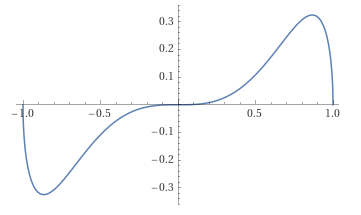
\includegraphics{images/grafica1.png}}}
                \end{center}

                Observando la función, podemos observar que es impar, esto se puede verificar ya que

                $$ - (x^3\sqrt{1-x^2}) = (-x)^3\sqrt{1-(-x)^2}$$

                Luego $\int_{-1}^{1}x^3\sqrt{1-x^2}dx = 0$, esto se puede observar gráficamente ya que el área debajo del eje $x$ es igual al área sobre el eje, por lo cual se cancelan.

                \item $\int_{-1}^{1}(x^5+3)\sqrt{1-x} dx$

                Primero manipulemos la expresión para que sea más fácil de trabajar,

                $$\int_{-1}^{1}(x^5+3)\sqrt{1-x}dx = \int_{-1}^{1}x^5\sqrt{1-x}dx + \int_{-1}^{1}3\sqrt{1-xdx}$$

                Observemos que $x^5\sqrt{1-x}$ es impar, por lo tanto $\int_{-1}^{1}x^5\sqrt{1-x} = 0$. Además observemos que $\sqrt{1-xdx}$ es una función par, por lo tanto  $\int_{-1}^{1}\sqrt{1-xdx} = 2\int_{0}^{1}\sqrt{1-xdx}$. Por último observemos que $\sqrt{1-x}$ es la función del círculo unitario, por lo tanto $\int_{0}^{1}\sqrt{1-xdx} = \pi/4$  así tenemos los siguiente

                \begin{align*}
                    \int_{-1}^{1}(x^5+3)\sqrt{1-x}dx &= \int_{-1}^{1}x^5\sqrt{1-x}dx + \int_{-1}^{1}3\sqrt{1-xdx}\\
                    &= 0 + 3\int_{-1}^{1}\sqrt{1-xdx}\\
                    &= 6\int_{0}^{1}\sqrt{1-xdx}\\
                    &= 6 \left(\dfrac{\pi}{4}\right)\\
                    &= \dfrac{3\pi}{4}
                \end{align*}
            \end{enumerate}
            \setcounter{enumi}{6}
            \item Decidir cuáles de las siguientes funciones siguientes son integrables sobre $[0,2]$, y calcular la integral cuando sea posible.
            \begin{enumerate}
                \item $f(x) = \begin{cases}
                    x, & 0\leq x < 1\\
                    x-2, & 1\leq x \leq 2
                \end{cases}$

                La función es integrable y su integral se calcula de la siguiente manera

                \begin{align*}
                    \int_{0}^{2}f(x)dx &= \int_{0}^{1}xdx + \int_{1}^{2}x-2dx\\
                    &= \int_{0}^{1}xdx + \int_{1}^{2}x -\int_{1}^{2}2dx\\
                    &= \left(\dfrac{1^2}{2} - \dfrac{0^2}{2}\right) + \left(\dfrac{2^2}{2} - \dfrac{1^2}{2}-2(2-1)\right)\\
                    &= \dfrac{1}{2} + 2 - \dfrac{1}{2} - 4 + 2\\
                    &= 0
                \end{align*}

                \setcounter{enumii}{2}
                \item $f(x) = x + [x]$

                La función es integrable y su integral se calcula de la siguiente manera

                \begin{align*}
                    \int_{0}^{2}x+[x]dx &= \int_{0}^{2} xdx + \int_{0}^{2}[x]dx\\
                    &= \int_{0}^{2} xdx + \int_{0}^{1}[x]dx + \int_{1}^{2} [x] dx\\
                    &= \left(\dfrac{2^2}{2} - \dfrac{0^2}{2}\right) + 0(1-0) + 1(2-1)\\
                    &= 3
                \end{align*}

                \setcounter{enumii}{5}
                \item $f(x) = \begin{cases}
                    \dfrac{1}{\left[\dfrac{1}{x}\right]}, & 0 < x \leq 1\\
                    0, & x=0 \text{ o } x > 1
                \end{cases}$

                Analicemos los valores que toma nuestra función

                \begin{table}[H]
                    \setlength{\extrarowheight}{20pt}
                    \centering
                    \begin{adjustbox}{valign=c}
                    \begin{tabular}{|c|c|}
                        \hline
                        $\left[\dfrac{1}{x}\right]$ & Condición                           \\ \hline
                        $\dfrac{1}{1}$              & $1 \leq \dfrac{1}{x} < 2 \leftrightarrow \dfrac{1}{2} < x \leq 1$               \\ \hline
                        $\dfrac{1}{2}$              & $2 \leq \dfrac{1}{x} < 3 \leftrightarrow \dfrac{1}{3} < x \leq \dfrac{1}{2}$     \\ \hline
                        $\dfrac{1}{2}$              & $3 \leq \dfrac{1}{x} < 4 \leftrightarrow \dfrac{1}{4} < x \leq \dfrac{1}{3}$     \\ \hline
                        $\vdots$                    & $\vdots$                                                                       \\ \hline
                        $\dfrac{1}{n}$                & $n \leq \dfrac{1}{x} < n+1 \leftrightarrow \dfrac{1}{n+1} < x \leq \dfrac{1}{n}$ \\ \hline
                    \end{tabular}
                \end{adjustbox}
                \end{table}

                Con esta tabla de valores podemos obtener la siguiente gráfica\\
                \begin{center}
                    \fbox{\adjustbox{trim=1 1 1 1, width=.5\textwidth}{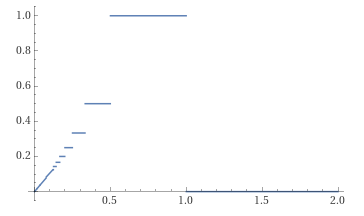
\includegraphics{images/grafica2.png}}}
                \end{center}

                Así, podemos dividir $(0, 1]$ en intervalos, obtener el área de esos intervalos y sumar las áreas. Haremos esto de la siguiente manera, primero veamos cuál es el área de los intervalos

                $$\int_{\dfrac{1}{2}}^{1} f(x)dx = 1(1-\dfrac{1}{2}) = \dfrac{1}{2}$$
                $$\int_{\dfrac{1}{3}}^{\dfrac{1}{2}} f(x)dx = \dfrac{1}{2}(\dfrac{1}{2} - \dfrac{1}{3}) = \dfrac{1}{12}$$
                $$\int_{\dfrac{1}{4}}^{\dfrac{1}{3}} f(x)dx = \dfrac{1}{3}(\dfrac{1}{3} - \dfrac{1}{4}) = \dfrac{1}{36}$$

                Luego, nuestra integral toma el siguiente valor

                \begin{align*}
                    \int_{0}^{2}f(x)dx &= \int_{0}^{1}f(x)dx + \int_{1}^{2}f(x)dx\\
                    &= \int_{0}^{1}f(x)dx + 0\\
                    &= 1(1-\dfrac{1}{2}) + \dfrac{1}{2}(\dfrac{1}{2} - \dfrac{1}{3}) + \dfrac{1}{3}(\dfrac{1}{3} - \dfrac{1}{4}) + \cdots\\
                    &= \sum_{n=1}^{\infty} \dfrac{1}{n^2(n+1)}\\
                    &= \frac{1}{6}(\pi^2-6)
                \end{align*}

                \item $f$ es la función indicada en la siguiente figura
                \begin{center}
                    \fbox{\adjustbox{trim=1 1 1 1, clip, width=0.7\textwidth}{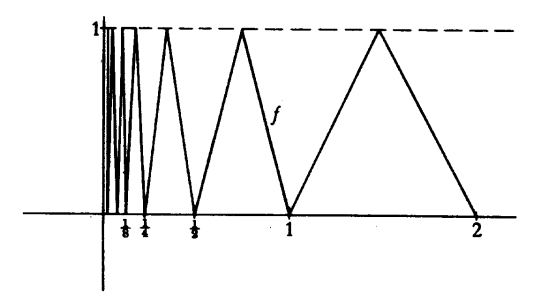
\includegraphics{images/grafica3.png}}}
                \end{center}

                Analicemos el área en cada intervalo en el cambia la función. En cada intervalo la función forma un triángulo, algunos intervalos en los que podemos observar que cambia la función son $[1,2]$, $[\frac{1}{2}, 1$], $[\frac{1}{4}, \frac{1}{2}]$, $[\frac{1}{8}, \frac{1}{4}]$.

                $\int_{1}^{2}f(x)dx = \frac{1(2-1)}{2} = \frac{1}{2}$
                Para el intervalo $[\frac{1}{2}, 1]$, el área del triángulo es:

                \[
                \int_{\frac{1}{2}}^{1} f(x) \, dx = \frac{1 (1-\frac{1}{2})}{2} = \frac{1}{4}
                \]

                Para el intervalo $[\frac{1}{4}, \frac{1}{2}]$, el área del triángulo es:

                \[
                \int_{\frac{1}{4}}^{\frac{1}{2}} f(x) \, dx = \frac{1 (\frac{1}{2}-\frac{1}{4})}{2} = \frac{1}{8}
                \]

                Finalmente, para el intervalo $[\frac{1}{8}, \frac{1}{4}]$, el área del triángulo es:

                \[
                \int_{\frac{1}{8}}^{\frac{1}{4}} f(x) \, dx = \frac{1 (\frac{1}{4}-\frac{1}{8})}{2} = \frac{1}{16}
                \]

                Con esto tenemos que

                \begin{align*}
                    \int_{0}^{2} f(x)dx &= \int_{1}^{2}f(x)dx + \int_{\frac{1}{2}}^{1}f(x)\,dx + \int_{\frac{1}{4}}^{\frac{1}{2}}f(x)\,dx + \cdots\\
                    &= \frac{1}{2} + \frac{1}{4} + \frac{1}{8} + \cdots\\
                    &= \sum_{n=1}^{\infty}\frac{1}{2^n}\\
                    &= 1
                \end{align*}
            \end{enumerate}

            \item Hallar las áreas de las regiones limitadas por
            \begin{enumerate}
                \setcounter{enumii}{2}
                \item Las gráficas de $f(x) = x^2$ y $g(x) = 1 - x^2$
                \begin{center}
                    \fbox{\adjustbox{trim=1 1 1 1, width=.5\textwidth}{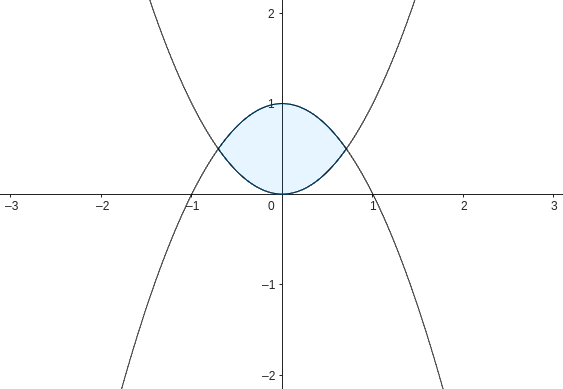
\includegraphics{images/grafica4.png}}}
                \end{center}

                Consideraremos el intervalo $[-1, 1]$, sabemos que la altura va a ser $h = (2-x^2)-x^2$, luego

                \begin{align*}
                    A &= \int_{-1}^{1}1-2x^2\,dx\\
                    &= \int_{-1}^{1}1\,dx - \int_{-1}^{1}2x^2\,dx\\
                    &= \left. x - \frac{2^3}{x} \right|_{-1}^{1}\\
                    &= \frac{2}{3}
                \end{align*}
                \setcounter{enumii}{5}
                \item La gráfica de $f(x) = \sqrt{x}$, el eje horizontal y la vertical por $(2, 0)$.
                La gráfica de la función es la siguiente

                \begin{center}
                    \fbox{\adjustbox{trim=1 1 1 1, width=.7\textwidth}{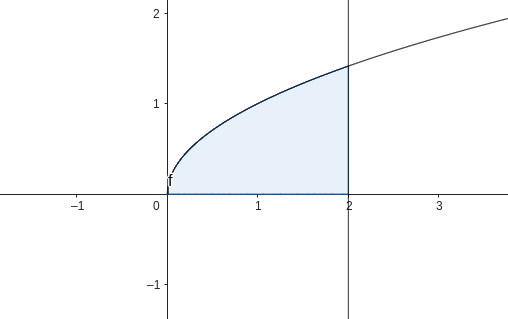
\includegraphics{images/grafica5.png}}}
                \end{center}

            \end{enumerate}
            \item Hallar
            $$\int_{a}^{b}\left(\int_{c}^{d}f(x)g(y)dy\right)$$
            en términos de $\int_{a}^{b}f$ y $\int_{a}^{b}g$.

            Para esto, consideraremos las constantes que están dentro de las integrales, observemos que en integral de adentro, $f(x)$ sería una constante ya que se está integrando con respecto a $y$ y no a $x$. Así, tenemos

            \begin{align*}
                \int_{a}^{b}\left(\int_{c}^{d}f(x)g(y)dy\right)\, dx &= \int_{a}^{b}f(x)\left(\int_{c}^{d}g(y)\, dy\right)\, dx
            \end{align*}

            Observemos ahora que la integral de adentro es constante con respecto a la integral de afuera, así se puede concluir lo siguiente

            \begin{align*}
                \int_{a}^{b}f(x)\left(\int_{c}^{d}g(y)\, dy\right)\, dx &= \int_{c}^{d}g(y)\,dy \int_{a}^{b}f(x)\,dx
            \end{align*}

            \setcounter{enumi}{12}
            \item Si $a < b < c < d$ y $f$ es integrable sobre $[a, d]$, demostrar que $f$ es integrable sobre $[b,c]$.

            Para el ejercicio usaremos el Teorema 4. Como $a < b < c < d$, tenemos que $a<c<d$ y como $f$ es integrable sobre $[a, d]$, por el Teorema 4 tenemos que $f$ es integrable sobre $[a,c]$ y sobre $[c,d]$. Luego, como $a<b<c$, aplicando nuevamente el Teorema 4 tenemos que $f$ es integrable sobre $[b, c]$.

            \setcounter{enumi}{19}
            \item Supongamos que $f$ está acotada sobre $[a,b]$ y que $f$ es continua en todo punto de $[a,b]$ con la excepción de $x_0$ de $(a,b)$. Demostrar que $f$ es integrable sobre $[a,b]$.

            Primero definamos las siguientes funciones

            $$f_1(x) = \begin{cases}
                f(x), & x<x_0\\
                0, & x>x_0\\
                m, & x = x_0
            \end{cases}$$

            Donde $m = \lim_{x \to x_0^-} f(x)$

            $$f_2(x) = \begin{cases}
                f(x), & x>x_0\\
                0, & x<x_0\\
                n, & x = x_0
            \end{cases}$$

            Donde $n = \lim_{x \to x_0^+} f(x)$. Y sea

            $$f_3(x) = \begin{cases}
                0, & x\not=x_0\\
                f(x_0)-m-n, & x=x_0\\
            \end{cases}$$

            Luego $f = f_1 + f_2 + f_3$, como $f_1, f_2, f_3$ son integrables, $f$ es integrable por el Teorema 5.
    \end{enumerate}
\end{document}
